\documentclass[conference]{IEEEtran}
\IEEEoverridecommandlockouts
% The preceding line is only needed to identify funding in the first footnote. If that is unneeded, please comment it out.
\usepackage{cite}
\usepackage{amsmath,amssymb,amsfonts}
\usepackage{algorithmic}
\usepackage{graphicx}
\usepackage{textcomp}
\usepackage[table,xcdraw]{xcolor}
\usepackage[utf8]{inputenc}
\usepackage[vietnamese]{babel}
\usepackage{float} 
\usepackage{multirow}
\usepackage{url}
\usepackage{amsmath}
\usepackage{graphicx}
\usepackage{tikz}

\usetikzlibrary{positioning, shapes.geometric, arrows.meta}

\bibliographystyle{IEEEtran}

\def\BibTeX{{\rm B\kern-.05em{\sc i\kern-.025em b}\kern-.08em
    T\kern-.1667em\lower.7ex\hbox{E}\kern-.125emX}}
\begin{document}

\title{DỰ BÁO MỨC ĐỘ CHỈ SỐ CHẤT LƯỢNG KHÔNG KHÍ TẠI BA THÀNH PHỐ CỦA VIỆT NAM SỬ DỤNG PHƯƠNG PHÁP HỌC MÁY VÀ HỌC SÂU\\
{\footnotesize}
\thanks{Identify applicable funding agency here. If none, delete this.}
}

\makeatletter
\newcommand{\linebreakand}{%
    \end{@IEEEauthorhalign}
    \hfill\mbox{}\par
    \mbox{}\hfill\begin{@IEEEauthorhalign}
}
\makeatother

\author{
    \IEEEauthorblockN{1\textsuperscript{st} Cao Hoài Sang}
    \IEEEauthorblockA{
        \textit{Khoa Hệ Thống Thông Tin}\\
        TP.HCM, Việt Nam \\
        21522541@gm.uit.edu.vn}
    \and
    \IEEEauthorblockN{2\textsuperscript{nd} Nguyễn Trần Gia Kiệt}
    \IEEEauthorblockA{
        \textit{Khoa Hệ Thống Thông Tin}\\
        TP.HCM, Việt Nam \\
        21522258@gm.uit.edu.vn}
    \and
    \IEEEauthorblockN{3\textsuperscript{rd} Thi Thành Công}
    \IEEEauthorblockA{
        \textit{Khoa Hệ Thống Thông Tin}\\
        TP.HCM, Việt Nam \\
        21521897@gm.uit.edu.vn}
    \linebreakand
    \IEEEauthorblockN{4\textsuperscript{th} Nguyễn Hoàng Đăng Khoa}
    \IEEEauthorblockA{
        \textit{Khoa Hệ Thống Thông Tin}\\
        TP.HCM, Việt Nam \\
        21520999@gm.uit.edu.vn}
    \and
    \IEEEauthorblockN{5\textsuperscript{th} Cù Ngọc Hoàng}
    \IEEEauthorblockA{
        \textit{Khoa Hệ Thống Thông Tin}\\
        TP.HCM, Việt Nam \\
        21522086@gm.uit.edu.vn}
}

\maketitle

\begin{abstract}
    Mục tiêu chính của nghiên cứu này là dự đoán chất lượng không khí tai ba thành phố được chỉ định (Hà Nội, Việt Trì và Đà Nẵng) của Việt Nam bằng cách kết hợp các thuật toán học máy và học sâu. Các mô hình bao gồm Gauss Newton Method Non-Linear, Residual Convolutional Neural Networks (ResCNN), Neural Hierarchical Interpolation for Time Series Forecasting (N-HiTS), Dynamic Linear Model (DLM), Simple Exponential Smoothing (SES), Linear Regression (LR), Autoregressive Integrated Moving Average (ARIMA), Recurrent Neural Network (RNN), Gated Recurrent Unit (GRU), Long Short Term Memory (LSTM). Hiệu quả của tất cả các mô hình được đề cập trên được đo lường bằng Mean Absolute Percentage Error (MAPE), Root Mean Squared Error, nhằm đạt được độ chính xác tối đa trong dự báo chuỗi thời gian chất lượng không khí chính xác.
\end{abstract}

\begin{IEEEkeywords}
    Nonlinear regression, Gauss-Newton, generalized least squares, iteratively reweighted least
    squares
\end{IEEEkeywords}

\section{Giới Thiệu}
Với sự gia tăng dân số nhanh chóng ở Việt Nam cùng với sự công nghiệp hóa ngày càng mạnh mẽ ở các khu vực trọng yếu, vấn đề chất lượng không khí nhanh chóng trở thành mối quan tâm chính, đặc biệt là ở các thành phố lớn của Việt Nam. Sự suy giảm chất lượng không khí không chỉ gây ra những rủi ro lớn đối với sức khỏe của cư dân mà còn đe dọa sự cân bằng sinh thái mong manh của khu vực. Trong bối cảnh này, việc dự đoán chính xác và kịp thời các mức độ chất lượng không khí là rất cần thiết cho các chiến lược giảm thiểu hiệu quả và can thiệp y tế công cộng. Nghiên cứu của nhóm chúng tôi sử dụng sự kết hợp của các mô hình học máy và học sâu để dự đoán chất lượng không khí, bằng cách tận dụng sức mạnh của các thuật toán phức tạp như Gauss Newton Method Non-Linear, Resilient Convolutional Neural Networks (ResCNN), Neural Basis Expansion Analysis for Time Series Forecasting (N-BEATS), Dynamic Linear Model (DLM), Simple Exponential Smoothing (SES), Linear Regression (LR), Autoregressive Integrated Moving Average (ARIMA), Recurrent Neural Network (RNN), Gated Recurrent Unit (GRU), và Long Short Term Memory (LSTM).

Việc bao gồm một tập hợp đa dạng các mô hình cho phép chúng tôi khám phá các khía cạnh khác nhau của dữ liệu và so sánh hiệu suất của các phương pháp khác nhau. Chẳng hạn, các mô hình thống kê truyền thống như SES, LR, và ARIMA cung cấp tính giải thích và sự đơn giản, làm cho chúng trở thành các mô hình cơ sở có giá trị để so sánh. Mặt khác, các kiến trúc học sâu như RNN, GRU, và LSTM xuất sắc trong việc nắm bắt các phụ thuộc phi tuyến tính và phụ thuộc thời gian dài hạn, những đặc điểm thường có trong dữ liệu chuỗi thời gian chất lượng không khí. Ngoài ra, các phương pháp sáng tạo như ResCNN và N-HiTS mang lại những lợi thế độc đáo trong việc xử lý các cấu trúc không gian và thứ bậc trong dữ liệu, nâng cao độ chính xác của các dự đoán.

\section{Nghiên cứu liên quan}

\subsection{Gauss-Newton nonlinear method}

Vào năm 2023 , Gauss-Newton được ứng dụng để tối ưu hóa một biến thể của sai phân bình phương trung bình Bellman (MSBE). Cụ thể, Gauss-Newton được sử dụng trong mỗi vòng lặp của phương pháp học Tăng Cường Sai Phân Gauss-Newton (Gauss-Newton Temporal Difference - GNTD) để thực hiện các bước cập nhật tham số của mô hình xấp xỉ hàm phi tuyến.\cite{b1}

\subsection{ResCNN}
Phân loại ECG bằng bộ Ensemble của Residual CNNs với Cơ chế Chú ý.

Trong phân loại ECG, sử dụng ResNet kết hợp với cơ chế chú ý đa đầu đã chứng minh hiệu quả. Giải pháp của Đội ISIBrno-AIMT trong Cuộc thi PhysioNet 2021 đã thể hiện sự vượt trội bằng việc phân loại ECG thành 26 nhóm khác nhau. Phương pháp này tích hợp các hàm mất mát và tối ưu hóa tiến hóa, mang lại đóng góp quan trọng cho lĩnh vực này. \cite{b4}

\subsection{Dynamic linear models}
Tháng 2 năm 2001, Monica Chioga cùng với Carlo Gaetan từ Università di Padova, Ý đã đề xuất mô hình hóa các tác động của phơi nhiễm chất ô nhiễm ngắn hạn lên sức khỏe bằng cách sử dụng các mô hình tuyến tính tổng quát động, nhằm tìm ra mối quan hệ giữa số ca tử vong không do tai nạn hàng ngày và ô nhiễm không khí ở thành phố Birmingham, Alabama. \cite{b5}

Hiểu biết về động lực trong vành đai bức xạ là rất quan trọng. Các electron có năng lượng cao có thể gây hại cho các vệ tinh. Do đó, việc cung cấp cho các nhà vận hành vệ tinh dự báo chính xác về cường độ dòng electron với thời gian dự báo có thể hành động là rất quan trọng. Vì vậy, vào năm 2014, D. Osthus, P. C. Caragea, D. Higdon, S. K. Morley, G.D. Reeves, và B. P. Weaver đã sử dụng các mô hình tuyến tính động để dự báo electron trong vành đai bức xạ bằng cách so sánh độ chính xác dự báo trước 1 ngày của một mô hình tuyến tính động đơn giản với mô hình dự báo electron tương đối hiện tại (REFM). \cite{b6}

\subsection{N-BEATS}
Năm 2022, một nhóm gồm năm nhà nghiên cứu, sau khi xem xét các phương pháp dự báo chuỗi thời gian truyền thống như VAR và các biến thể của nó, nhận thấy chúng không hiệu quả do tính chất không ổn định của dữ liệu chất lượng không khí. Do đó, họ đã chọn sử dụng kiến trúc N-BEATS \cite{b8} để xây dựng mô hình dự báo cho nhiều chất ô nhiễm không khí khác nhau ở Thành phố Hồ Chí Minh, cụ thể là giá trị của NO2, SO2, CO và O3.

Năm 2021, một nhóm nghiên cứu tại Đại học Khoa học và Công nghệ Hà Nội và Đại học FPT đã áp dụng mô hình NBEATS để dự báo nhu cầu điện ngắn hạn ở Việt Nam \cite{b9}. 

\subsection{Recurrent Neural Network}
Trong nghiên cứu về hiểu biết ô nhiễm không khí, Brian S. Freemana, Graham Taylora, Bahram Gharabaghia, và Jesse Thé từ Trường Kỹ thuật, Đại học Guelph, Guelph, Ontario, Canada dự báo chuỗi thời gian chất lượng không khí bằng cách sử dụng mô hình học sâu mạng nơ-ron hồi quy (RNN) với bộ nhớ dài hạn (LSTM). \cite{b10}

\subsection{SES}
Nhóm tác giả từ University of Karachi, Pakistan đã sử dụng mô hình ARIMA và SES để dự đoán lượng khí thải CO2 từ một số nước châu Á như Japan, Bangladesh, China, Pakistan, India, Sri Lanka, Iran, Singapore, và Nepal trong khoảng từ năm 1971 đến 2014. Dựa trên FMAE, SES phù hợp để dự đoán lượng CO2 ở Pakistan và Sri Lanka. Trong khi đó, ARIMA thì phù hợp với Japan, China, India, Iran và Singapore. Đối với Nepal và Bangladesh, cả hai mô hình đều cho kết quả tương đương nhau. \cite{b11}


\subsection{Linear Regression}
Năm 2022, tại Đại học Manonmaniam Sundaranar, A. Loganathan, Sumithra Palraj, và Deneshkumar V đã công bố một nghiên cứu về việc sử dụng hồi quy tuyến tính để dự báo chỉ số Chất lượng không khí (AQI). Nghiên cứu tập trung vào phân tích dữ liệu AQI thu thập từ trạm giám sát ở Chennai, Ấn Độ, và xây dựng một mô hình hồi quy tuyến tính đa biến. Đánh giá về tính hợp lệ của mô hình được thực hiện thông qua phân tích dư thừa. \cite{b18}

\subsection{LSTM}
Ricardo Navares và José L. Aznarte đã sử dụng mô hình LSTM để dự đoán chất lượng không khí tại thành phố Marid. Nhóm tác giả dựa vào các chỉ số không khí gây hại như CO, NO2, O3, PM10, SO2 được thu thập tại các địa điểm khác nhau của Madrid. Sau đó sử dụng các cấu hình khác nhau của mô hình LSTM để dự đoán chất lượng không khí và so sánh cấu hình LSTM nào sẽ là tốt nhất. \cite{b12}

\subsection{ARIMA}
Hiện nay, hầu hết các nghiên cứu đều dựa trên việc dự đoán xu hướng thị trường chứng khoán bằng mạng nơ-ron dựa trên ARIMA \cite{b13} ARIMA được sử dụng làm cả mô hình phân tích và dự báo trong cơ sở dữ liệu PACAP‐CCER của Trung Quốc, được phát triển bởi Trung tâm Nghiên cứu Thị trường Vốn Thái Bình Dương (PACAP) tại Đại học Rhode Island (Mỹ) và Công ty Dịch vụ Thông tin SINOFIN, liên kết với Trung tâm Nghiên cứu Kinh tế Trung Quốc (CCER) của Đại học Bắc Kinh (Trung Quốc). \cite{b14} ARIMA đã được áp dụng để giải quyết các vấn đề thực tế trong thị trường chứng khoán bằng cách dự báo giá cổ phiếu của bốn công ty hàng đầu trong chỉ số Nifty Midcap-50 bằng MATLAB kèm theo các chỉ số hiệu suất. \cite{b15} Kết hợp mô hình hồi quy mờ và mô hình ARIMA, mô hình ARIMA mờ (FARIMA) đã được phát triển để dự đoán tỷ giá đồng Đài tệ sang Đô la Mỹ. \cite{b16} Một mục đích khác mà mô hình ARIMA đã được sử dụng là để dự đoán hoặc dự báo giá cả, cụ thể là giá điện của ngày mai.

\section{Tài nguyên}
\subsection{Bộ dữ liệu}
Dự báo chất lượng không khí là rất quan trọng để giảm thiểu các tác động tiêu cực của ô nhiễm lên sức khỏe con người và môi trường. Phân tích chuỗi thời gian nổi lên như một công cụ mạnh mẽ trong lĩnh vực này, cho phép dự đoán các mức độ chất lượng không khí trong tương lai dựa trên dữ liệu lịch sử.

Do các vấn đề phổ biến liên quan đến bụi mịn ở khu vực phía Bắc, nhóm đã chọn một bộ dữ liệu chi tiết về chất lượng không khí của ba thành phố lớn ở miền Bắc Việt Nam: Bắc Ninh, Hà Nội và Quảng Ninh.

Bộ dữ liệu chủ yếu kéo dài từ năm 2021 đến năm hiện tại, 2024, bao gồm 6 cột tương ứng với các thành phần khác nhau trong không khí và chất lượng không khí được đánh giá thông qua Chỉ số Chất lượng Không khí (AQI): nồng độ PM2.5, nồng độ PM10, nồng độ O3, nồng độ NO2, nồng độ SO2 và nồng độ CO.
\subsection{Thống kế mô tả}

\begin{table}[H]
    \centering
    \caption{HaNoi, DaNang, VietTri’s Descriptive Statistics}
    \begin{tabular}{|>{\columncolor{red!20}}c|c|c|c|}
        \hline
        \rowcolor{red!20} & HaNoi  & DaNang & VietTri \\ \hline
        Count             & 2840   & 3136   & 2348    \\ \hline
        Mean              & 75.351 & 78.721 & 60.160  \\ \hline
        Std               & 42.285 & 73.749 & 41.381  \\ \hline
        Min               & 11     & 13     & 15      \\ \hline
        25\%              & 43.0   & 43.0   & 31.0    \\ \hline
        50\%              & 66.0   & 59.0   & 47.0    \\ \hline
        75\%              & 101.0  & 88.0   & 81.0    \\ \hline
        Max               & 498    & 500    & 828     \\ \hline
    \end{tabular}
\end{table}

\begin{figure}[H]
    \centering
    \begin{minipage}{0.23\textwidth}
        \centering
        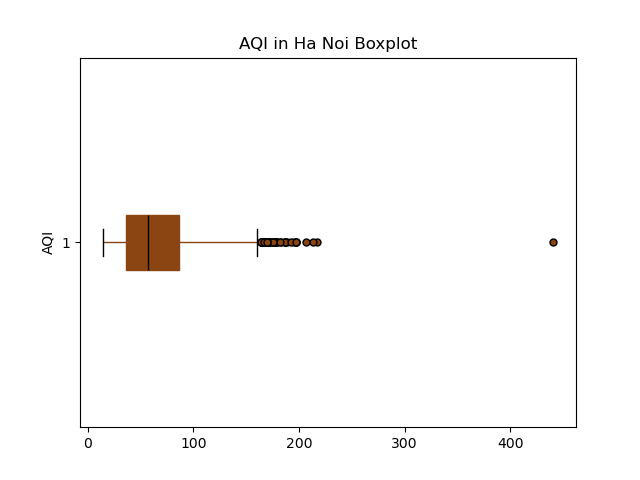
\includegraphics[width=1\textwidth]{bibliography/figure/Analysis-Dataset/BoxplotHaNoi.png}
        \caption{HaNoi AQI's boxplot}
        \label{fig:1}
    \end{minipage}
    \hfill
    \begin{minipage}{0.23\textwidth}
        \centering
        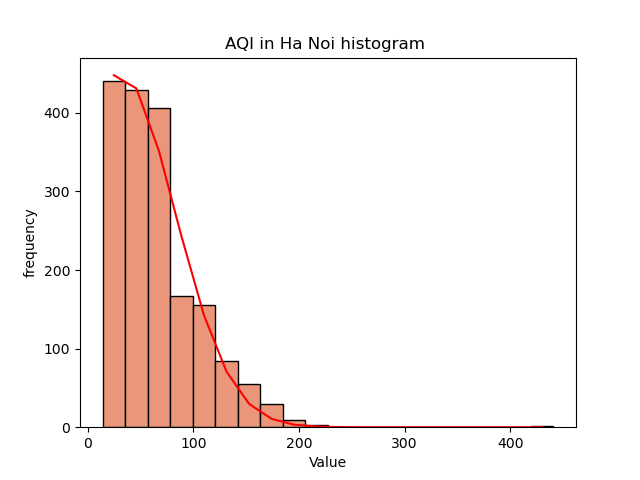
\includegraphics[width=1\textwidth]{bibliography/figure/Analysis-Dataset/histogramHaNoi.png}
        \caption{HaNoi AQI's histogram}
        \label{fig:2}
    \end{minipage}
\end{figure}

\begin{figure}[H]
    \centering
    \begin{minipage}{0.23\textwidth}
        \centering
        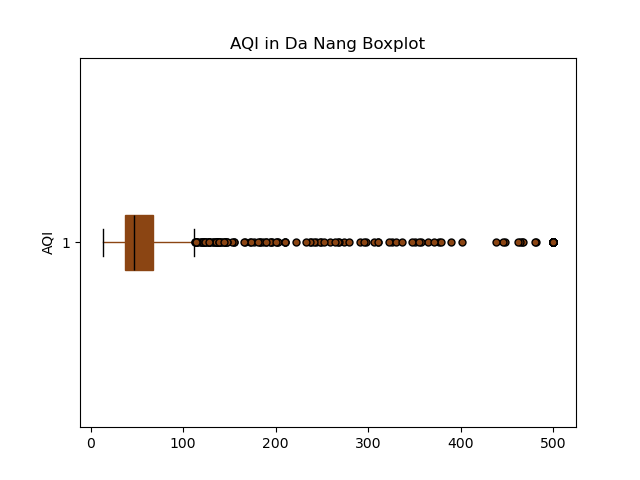
\includegraphics[width=1\textwidth]{bibliography/figure/Analysis-Dataset/BoxplotDaNang.png}
        \caption{DaNang AQI's boxplot}
        \label{fig:1}
    \end{minipage}
    \hfill
    \begin{minipage}{0.23\textwidth}
        \centering
        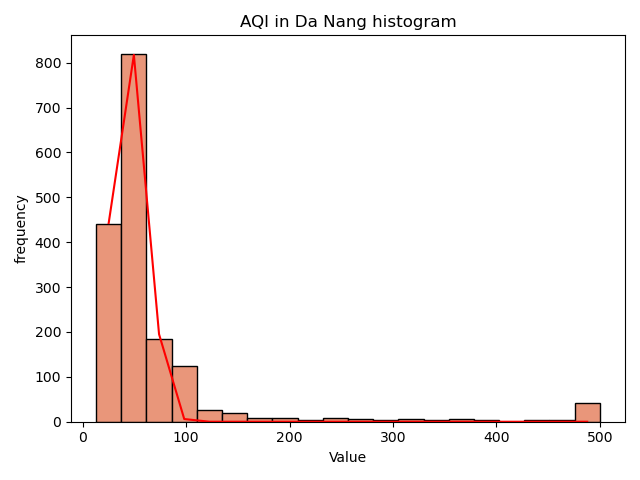
\includegraphics[width=1\textwidth]{bibliography/figure/Analysis-Dataset/histogramDaNang.png}
        \caption{DaNang AQI's histogram}
        \label{fig:2}
    \end{minipage}
\end{figure}

\begin{figure}[H]
    \centering
    \begin{minipage}{0.23\textwidth}
        \centering
        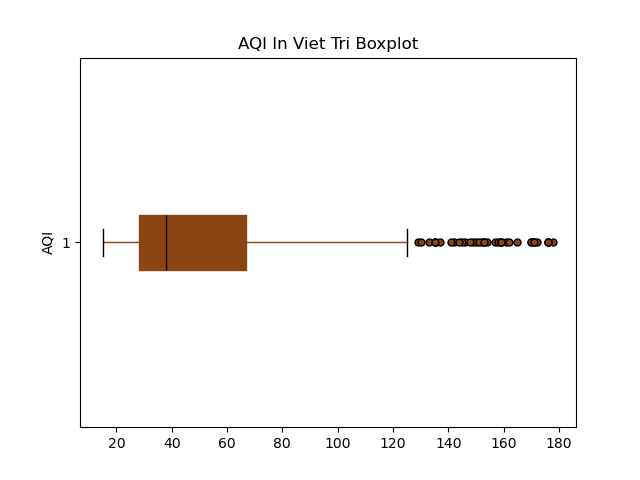
\includegraphics[width=1\textwidth]{bibliography/figure/Analysis-Dataset/BoxplotVietTri.png}
        \caption{VietTri AQI's boxplot}
        \label{fig:1}
    \end{minipage}
    \hfill
    \begin{minipage}{0.23\textwidth}
        \centering
        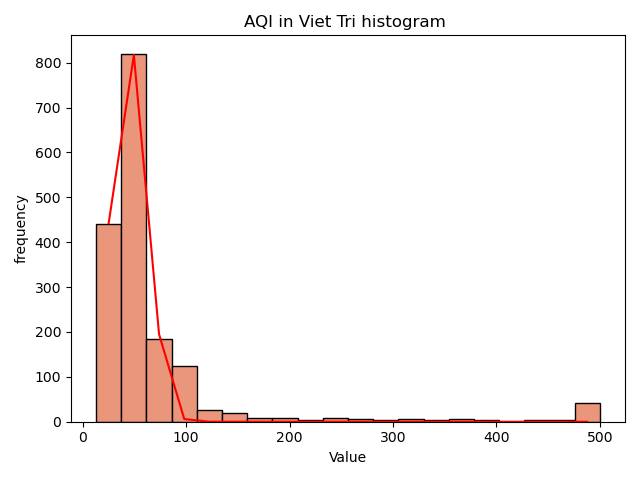
\includegraphics[width=1\textwidth]{bibliography/figure/Analysis-Dataset/histogramVietTri.png}
        \caption{VietTri AQI's histogram}
        \label{fig:2}
    \end{minipage}
\end{figure}

\section{Phương pháp luận}
\subsection{Gauss newton method nonlinear}

\subsubsection{Phương pháp Newton}
Với hàm \( y = y_0 e^{-kt} \), chúng ta tìm giá trị nhỏ nhất của SSE. Chúng ta tìm giá trị \(k\) bằng phương pháp Newton.

\begin{center}
    $SSE = \sum_{i}^{n}(y_i - y_0 e^{-kt_i})^2$
\end{center}

\begin{center}
    \(k_{\text{new}} = k_{\text{old}} - \frac{f'(k_{\text{old}})}{f''(k_{\text{old}})}\)
\end{center}

Hoặc chúng ta có thể giải thích bằng ma trận Hessian như sau:

\begin{center}
    \[
        \begin{pmatrix}
            k_{\text{new}} \\ y_{0,\text{new}}
        \end{pmatrix} =
        \begin{pmatrix}
            k_{\text{old}} \\ y_{0,\text{old}}
        \end{pmatrix} - H^{-1}G
    \]
\end{center}

Trong đó: \\
\indent\textbullet\ \(H = \begin{bmatrix}
    \frac{\partial^2 f}{\partial k^2}            & \frac{\partial^2 f}{\partial k \partial y_0} \\
    \frac{\partial^2 f}{\partial y_0 \partial k} & \frac{\partial^2 f}{\partial y_0^2}
\end{bmatrix}\)\\
\indent\textbullet\ \(G = \begin{bmatrix}
    \frac{\partial f}{\partial k} \\ \frac{\partial f}{\partial y_0}
\end{bmatrix}\)\\

Vấn đề với phương pháp Newton trong hồi quy phi tuyến là việc tính toán ma trận Hessian và nghịch đảo của nó gặp khó khăn. Để giải quyết vấn đề này, phương pháp Gauss-Newton thay thế bằng cách xấp xỉ ma trận Hessian.

Chúng ta có thể viết lại SSE như sau:
\begin{center}
    $SSE = \sum_{i}^{n}r_i^2 = r^T r$
\end{center}

Trong đó: \\
\indent\textbullet\ \(r\) là một vector chứa các sai số dư \\

\subsubsection{Phương pháp Gauss-Newton}
Chúng ta lấy đạo hàm của SSE theo các tham số trong mô hình bằng quy tắc chuỗi, chúng ta có được phương trình sau:
\begin{center}
    \(
    \frac{\partial SSE}{\partial \beta_j} = 2\sum_{i}^{n} r_i \frac{\partial r_i}{\partial \beta_j}
    \)
\end{center}

Sau đó, bỏ số hai vì nó sẽ không ảnh hưởng đến việc ước tính các tham số. Tương ứng với ma trận Jacobian.

\begin{center}
    \(
    J_r = \begin{bmatrix}
        \frac{\partial r_1}{\partial \beta_1} & \frac{\partial r_1}{\partial \beta_2} \\
        \frac{\partial r_2}{\partial \beta_1} & \frac{\partial r_2}{\partial \beta_2} \\
        \vdots                                & \vdots                                \\
        \frac{\partial r_n}{\partial \beta_1} & \frac{\partial r_n}{\partial \beta_2}
    \end{bmatrix}
    \)
\end{center}

Với phương trình sau cho tổng các sai số bình phương (SSE):
\[
    SSE = \sum_{i=1}^{n} (y_i - y_0 e^{-kt_i})^2
\]
Chúng ta có:
\begin{center}
    \(
    \frac{\partial^2 {SSE}}{\partial \beta_j \partial \beta_k} = \sum_{i}^{n} \left( \frac{\partial r_i}{\partial \beta_j} \frac{\partial r_i}{\partial \beta_k} + r_i \frac{\partial^2 r_i}{\partial \beta_j \partial \beta_k} \right)
    \)
\end{center}

Sự khác biệt chính giữa phương pháp Newton và Gauss-Newton là phương pháp Gauss-Newton bỏ qua \(r_i \frac{\partial^2 r_i}{\partial \beta_j \partial \beta_k}\).
Do đó, đạo hàm bậc hai được xấp xỉ bằng hàm sau:
\begin{center}
    \(
    \frac{\partial^2 {SSE}}{\partial \beta_j \partial \beta_k} \approx \sum_{i}^{n} \left( \frac{\partial r_i}{\partial \beta_j} \frac{\partial r_i}{\partial \beta_k} \right) = J^T_r J_r
    \)
\end{center}

Sử dụng quy tắc cập nhật sau trong phương pháp Newton. Đối với Gauss-Newton, đơn giản chỉ cần cắm vào xấp xỉ cho ma trận Hessian và gradient.

\begin{center}
    \[
        \begin{pmatrix}
            k_{\text{new}} \\ y_{0,\text{new}}
        \end{pmatrix} =
        \begin{pmatrix}
            k_{\text{old}} \\ y_{0,\text{old}}
        \end{pmatrix} - (J^T_r J_r)^{-1} J^T_r r
    \]
\end{center}

Với \(\beta\) là một vector cột với các tham số được ước tính. Đối với ví dụ đơn giản chỉ ước tính hai tham số, phương trình trông như sau:

\begin{center}
    \[
        \beta_{\text{new}} = \beta_{\text{old}} - (J^T_r J_r)^{-1} J^T_r r(\beta_{\text{old}})
    \]
    \[
        \begin{pmatrix}
            k_{\text{new}} \\ y_{0,\text{new}}
        \end{pmatrix} =
        \begin{pmatrix}
            k_{\text{old}} \\ y_{0,\text{old}}
        \end{pmatrix} - (J^T_r J_r)^{-1} J^T_r r \begin{pmatrix}
            k_{\text{old}} \\ y_{0,\text{old}}
        \end{pmatrix}
    \]
\end{center}
\vspace{3mm}
\subsection{AUTOREGRESSIVE INTEGRATED MOVING AVERAGE (ARIMA)}

ARIMA là viết tắt của "Autoregressive Integrated Moving Average". Mô hình ARIMA thường được sử dụng để dự báo dữ liệu chuỗi thời gian đơn biến. Mô hình ARIMA có thể xử lý một chuỗi thời gian nếu chuỗi đó là dừng và không có dữ liệu bị thiếu. Phương pháp này được sử dụng trong nhiều nghiên cứu để dự báo.

ARIMA là sự kết hợp của 3 thành phần, Auto-Regressive – AR, Integrated – I và Moving Average – MA tương ứng với các tham số p, d và q đại diện cho ba thành phần chính của mô hình, trong đó:
\\
\indent\textbullet\ \(p-AR(p)\): Tham số p đại diện cho số lượng các quá trình tự hồi quy trong thành phần tự hồi quy (AutoRegressive) của mô hình ARIMA. Nó chỉ ra số lượng ngày quá khứ của chuỗi dữ liệu mà được sử dụng để dự đoán giá trị hiện tại. Mỗi giá trị quá khứ được sử dụng là một hệ số trong mô hình tự hồi quy. Giá trị của p phụ thuộc vào sự phụ thuộc tạm thời trong chuỗi dữ liệu và có thể được xác định bằng cách sử dụng các phương pháp như đồ thị tự tương quan (ACF - AutoCorrelation Function) hoặc hàm tương quan một lệnh (PACF - Partial AutoCorrelation Function). Phương trình tự hồi quy AR được tổng quát như sau:\\
\[
    Y_t = c + \varphi_1 Y_{t-1} + \varphi_2 Y_{t-2} + \ldots + \varphi_p Y_{t-p} + \epsilon_t
\]
Trong đó: \\
\indent -- \(Y_t\) đại diện cho giá trị dữ liệu tại thời điểm t\\
\indent -- \(c\) là hằng số chặn\\
\indent -- \(\varphi\) là hệ số AutoRegressive(AR)\\
\indent -- \(\epsilon_t\) là sai số ngẫu nhiên \\
\indent -- \(p\) là số bậc \\

\indent\textbullet\ \(q-MA(q)\): Tham số q đại diện cho số lượng các thành phần trung bình động (Moving Average) trong mô hình ARIMA. Nó chỉ ra số lượng giá trị trung bình động được sử dụng để dự đoán giá trị hiện tại.\\
\[
    Y_t = c + \theta_1 \epsilon_{t-1} + \theta_2 \epsilon_{t-2} + \ldots + \theta_p \epsilon_{t-p} + \epsilon_t
\]

Trong đó: \\
\indent -- \(Y_t\) đại diện cho giá trị dữ liệu tại thời điểm t\\
\indent -- \(c\) là hằng số chặn\\
\indent -- \(\theta\) là hệ số Moving Average(MA)\\
\indent -- \(\epsilon_t\) là hệ số tương quan\\
\indent -- \(p\) là số bậc \\

\indent\textbullet\  \(d-I(d)\): Tham số d đại diện cho số lần lấy đạo hàm-sai phân (differencing) trên chuỗi dữ liệu ban đầu để loại bỏ xu hướng (trend) và/hoặc thành phần mùa vụ (seasonality) hay chuyển đổi dữ liệu thành chuỗi dừng. chuỗi dừng là chuỗi có trung bình, phương sai và tự tương quan không đổi theo thời gian. Một chuỗi thời gian được coi là chuỗi dừng nếu nó có trung bình không đổi, phương sai không đổi và tự tương quan không đổi. Chuỗi dừng là Công thức tính sai phân tại thời điểm t như sau
\[
    \Delta y_t = y_t - y_{t-1}
\]

Sau khi kết hợp tất cả, ta có ARIMA(p, d, q) được biểu diễn như sau:
\[
    \Delta y_t = c + \varphi_1 \Delta y_{t-1} + \ldots + \varphi_p \Delta y_{t-p} + \varepsilon_t + \theta_1 \varepsilon_{t-1} + \theta_1 \varepsilon_{t-1} + \ldots + \theta_q \varepsilon_{t-q}
\]

Trong đó: \\
\indent -- \(Y_t\) đại diện cho giá trị dữ liệu tại thời điểm t\\
\indent -- \(c\) là hằng số chặn\\
\indent -- \(\theta\) là hệ số Moving Average(MA)\\
\indent -- \(\epsilon_t\) là hệ số tương quan\\
\indent -- \(\varphi\) là hệ số AutoRegressive(AR)\\
\subsection{ResCNN}
\subsubsection{Tổng quan}
Mô hình ResCNN là một mô hình dự đoán chuỗi thời gian kết hợp giữa LSTM và CNN 1D sử dụng kết nối bỏ qua.

\subsubsection{ResCNN với cách tiếp cận dựa trên độ dốc}
\paragraph{Giới thiệu mô hình}
Chúng tôi đề xuất một mô hình ResCNN với kết nối dư trên các lớp CNN 1D, giúp tránh mất thông tin quan trọng khi áp dụng nhiều lớp tích chập liên tiếp.

\paragraph{Thiết kế mô hình}
\begin{figure}[H]
    \centering
    \begin{minipage}{0.23\textwidth}
        \centering
        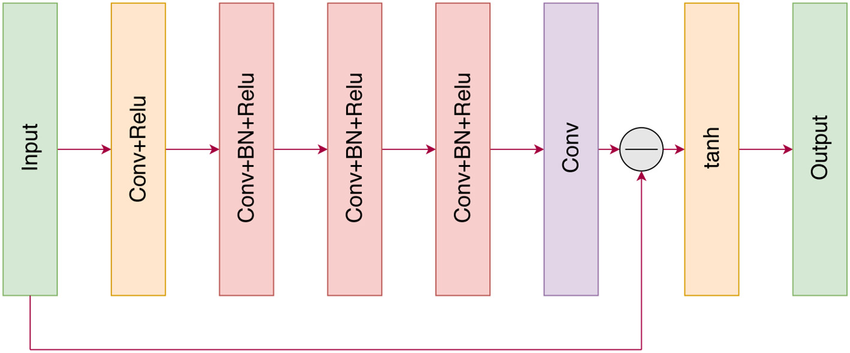
\includegraphics[width=1\textwidth]{bibliography/figure/ResCNN/ResCNN_1.png}
        \caption{Mô hình ResCNN được đề xuất}
        \label{fig:gru_del_up}
    \end{minipage}
\end{figure}

\paragraph{Các thành phần chính}
\begin{itemize}
    \item \textbf{Input}: Dữ liệu chuỗi thời gian đầu vào.
    \item \textbf{LSTM}: Xử lý và ghi nhớ thông tin tuần tự, nắm bắt mối quan hệ dài hạn.
    \item \textbf{Conv + ReLU}:
          \begin{itemize}
              \item \textbf{Conv}: Trích xuất đặc trưng không gian.
              \item \textbf{ReLU}: Học đặc trưng phi tuyến tính.
          \end{itemize}
    \item \textbf{Conv + BN + ReLU}:
          \begin{itemize}
              \item \textbf{Conv}: Tiếp tục trích xuất đặc trưng.
              \item \textbf{BN}: Chuẩn hóa theo batch, ổn định và tăng tốc huấn luyện.
              \item \textbf{ReLU}: Học đặc trưng phi tuyến tính.
          \end{itemize}
    \item \textbf{Conv}: Lớp tích chập cuối cùng không có hàm kích hoạt.
    \item \textbf{Skip Connection}: Bảo toàn thông tin từ đầu vào ban đầu.
    \item \textbf{Tanh}: Đưa đầu ra về khoảng giá trị [-1, 1].
    \item \textbf{Output}: Kết quả cuối cùng sau tất cả các lớp.
\end{itemize}

Tóm lại, mô hình này sử dụng các lớp tích chập để trích xuất đặc trưng phức tạp, ReLU và chuẩn hóa theo batch tăng tính phi tuyến và ổn định, kết nối tắt và tanh cải thiện hiệu quả học tập và chuẩn hóa đầu ra.

\subsubsection{1D-CNN}
CNN 1D được sử dụng trong xử lý ngôn ngữ tự nhiên và phân tích chuỗi thời gian, trích xuất đặc trưng bằng cách di chuyển kernel dọc theo trục thời gian. Công thức tổng quát:
\begin{multline}
    \text{out}(N_i, C_{out_j}, L_{out_l}) = \text{bias}(C_{out_j}) \\
    + \sum_{k=0}^{C_{in}-1} \text{weight}(C_{out_j}, k) \ast \text{input}(N_i, k, L_{l-k})
\end{multline}
\subsubsection{Lớp Chuẩn hóa Theo Batch}
Chuẩn hóa đầu ra của lớp tích chập để cải thiện huấn luyện:

\[
    \hat{x} = \frac{x - \mu}{\sqrt{\sigma^2 + \epsilon}}
\]

\subsubsection{Lớp kích hoạt cuối cùng}
Hàm kích hoạt \texttt{tanh} biến đổi đầu ra thành khoảng \((-1, 1)\):

\[
    \text{tanh}(x) = \frac{e^x - e^{-x}}{e^x + e^{-x}}
\]

\subsubsection{Kết nối còn lại}
Kết nối còn lại thêm đầu vào ban đầu vào đầu ra của lớp tích chập cuối cùng:

\[
    \textbf{out}_{res}(x) = x + \text{Conv}(x)
\]


\subsection{Gated Recurrent Unit (GRU)}
\subsubsection{GRU là gì?}
GRU là một biến thể của LSTM

Sự khác biệt chính giữa GRU và LSTM nằm ở cách xử lý trạng thái ẩn và ô nhớ:

\begin{itemize}
    \item \textbf{LSTM}: Sử dụng ba cổng (input gate, output gate và forget gate) để duy trì trạng thái của ô nhớ riêng biệt.
    \item \textbf{GRU}: Không có ô nhớ riêng biệt, thay vào đó, nó sử dụng một “vector kích hoạt ứng viên” và hai cổng (reset gate và update gate).
\end{itemize}

\begin{itemize}
    \item \textbf{Cổng thiết lập lại (reset gate)}: Quyết định bao nhiêu trạng thái ẩn trước đó cần quên.
    \item \textbf{Cổng cập nhật (update gate)}: Quyết định bao nhiêu của vector kích hoạt ứng viên cần tích hợp vào trạng thái ẩn mới.
\end{itemize}

\subsubsection{Cổng thiết lập lại và cổng cập nhật}
Đầu tiên ta giới thiệu thiết lập lại và cổng cập nhật. Ta thiết kế chúng thành các vector có các phần tử trong khoảng  (0,1)
để có thể biểu diễn các tổ hợp lồi. Chẳng hạn, một biến xóa cho phép kiểm soát bao nhiêu phần của trạng thái trước đây được giữ lại. Tương tự, một biến cập nhật cho phép kiểm soát bao nhiêu phần của trạng thái mới sẽ giống trạng thái cũ.


\begin{figure}[H]
    \centering
    \begin{minipage}{0.23\textwidth}
        \centering
        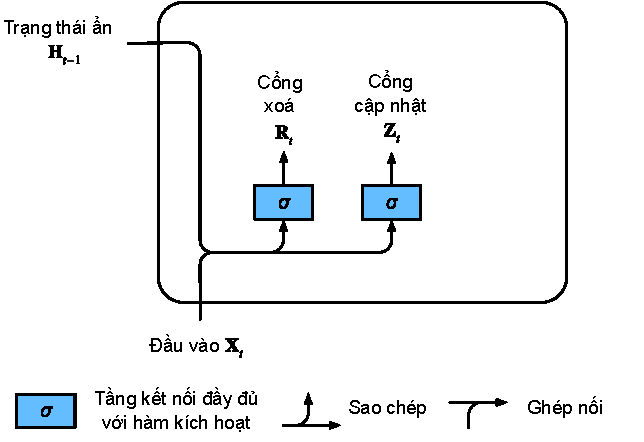
\includegraphics[width=1\textwidth]{bibliography/figure/GRU/gru_1.pdf}
        \caption{Cổng thiết lập lại và cổng cập nhật trong GRU}
        \label{fig:gru_del_up}
    \end{minipage}
\end{figure}

Ta bắt đầu bằng việc thiết kế các cổng tạo ra các biến này. Hình \ref{fig:gru_del_up}
minh họa các đầu vào cho cả cổng thiết lập lại và cổng cập nhật trong GRU, với đầu vào ở bước thời gian hiện tại  \(\mathbf{X}_t \)
và trạng thái ẩn ở bước thời gian trước đó  \(\mathbf{H}_{t-1} \). Đầu ra được tạo bởi một tầng kết nối đầy đủ với hàm kích hoạt sigmoid.

Tại bước thời gian $t$, với đầu vào là $\mathbf{X}_t \in \mathbb{R}^{n \times d}$ (số lượng mẫu: $n$, số lượng đầu vào: $d$) và trạng thái ẩn ở bước thời gian gần nhất là $\mathbf{H}_{t-1} \in \mathbb{R}^{n \times h}$ (số lượng trạng thái ẩn: $h$), cổng thiết lập lại $\mathbf{R}_t \in \mathbb{R}^{n \times h}$ và cổng cập nhật $\mathbf{Z}_t \in \mathbb{R}^{n \times h}$ được tính như sau:

\begin{equation*}
    \mathbf{R}_t = \sigma(\mathbf{X}_t \mathbf{W}_{xr} + \mathbf{H}_{t-1} \mathbf{W}_{hr} + \mathbf{b}_r)
\end{equation*}
\begin{equation*}
    \mathbf{Z}_t = \sigma(\mathbf{X}_t \mathbf{W}_{xz} + \mathbf{H}_{t-1} \mathbf{W}_{hz} + \mathbf{b}_z).
\end{equation*}

Ở đây, $\mathbf{W}_{xr}, \mathbf{W}_{xz} \in \mathbb{R}^{d \times h}$ và $\mathbf{W}_{hr}, \mathbf{W}_{hz} \in \mathbb{R}^{h \times h}$ là các ma trận trọng số và $\mathbf{b}_r, \mathbf{b}_z \in \mathbb{R}^{1 \times h}$ là các hệ số điều chỉnh. Ta sẽ sử dụng hàm sigmoid để biến đổi các giá trị đầu vào nằm trong khoảng $(0, 1)$.

\subsubsection{Hoạt động của cổng thiết lập lại}
Trong RNN thông thường, ta cập nhật trọng thái cổng thiết lập lại theo công thức
\[
    \mathbf{H}_t = \tanh(\mathbf{X}_t \mathbf{W}_{xh} + \mathbf{H}_{t-1} \mathbf{W}_{hh} + \mathbf{b}_h).
\]

Hình \ref{fig:gru_del} minh họa luồng tính toán sau khi áp dụng cổng thiết lập lại. Ký hiệu \(\bigodot\) biểu thị phép nhân theo từng phần tử giữa các tensor.

\begin{figure}[H]
    \centering
    \begin{minipage}{0.23\textwidth}
        \centering
        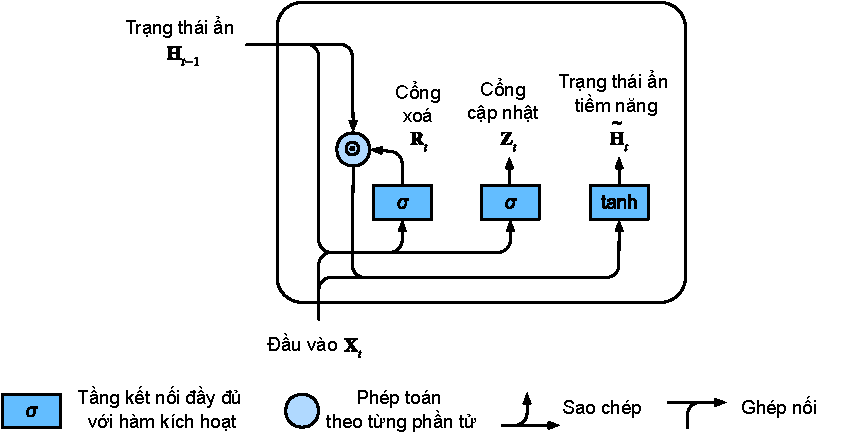
\includegraphics[width=1\textwidth]{bibliography/figure/GRU/gru_2.pdf}
        \caption{Tính toán trạng thái tiềm năng trong một GRU. Phép nhân được thực hiện theo phần tử}
        \label{fig:gru_del}
    \end{minipage}

\end{figure}

\begin{equation*}
    \tilde{\mathbf{H}}_t = \tanh (\mathbf{X}_t \mathbf{W}_{xh} + (\mathbf{R}_t \odot \mathbf{H}_{t-1}) \mathbf{W}_{hh} + \mathbf{b}_h).
\end{equation*}

\subsubsection{Hoạt động của cổng cập nhật}
Cổng này xác định mức độ giống nhau giữa trạng thái mới \(\mathbf{H}_t \) và trạng thái cũ \(\mathbf{H}_{t-1}\) cũng như mức độ trạng thái tiềm năng \(\widetilde{\mathbf{H}}_t\) được sử dụng. Cổng cập nhật \(\mathbf{Z}_t\) được sử dụng cho mục đích này bằng cách áp dụng tổ hợp lồi giữa trạng thái cũ và trạng thái tiềm năng. Ta có phương
trình cập nhật cuối cho GRU.

\begin{equation*}
    \mathbf{H}_t = \mathbf{Z}_t \circ \mathbf{H}_{t-1} + (1 - \mathbf{Z}_t) \circ \tilde{\mathbf{H}}_t.
\end{equation*}

\begin{figure}[H]
    \centering
    \begin{minipage}{0.23\textwidth}
        \centering
        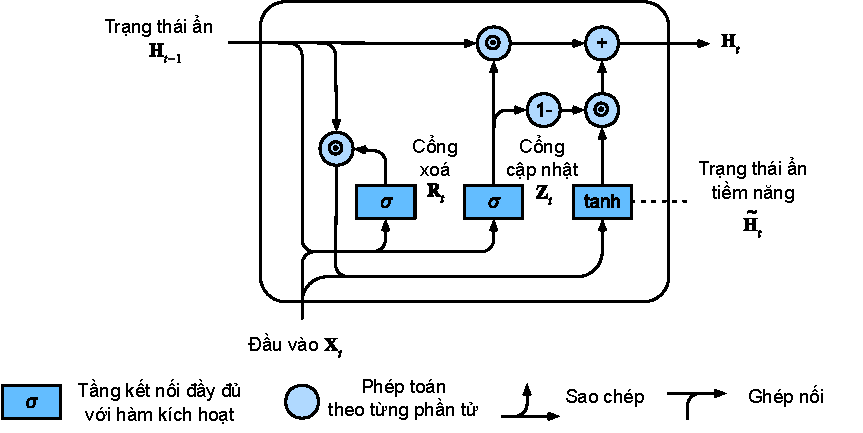
\includegraphics[width=1\textwidth]{bibliography/figure/GRU/gru_3.pdf}
        \caption{Tính toán trạng thái ẩn trong một GRU. Phép nhân được thực hiện cho từng phần tử}
        \label{fig:gru_up}
    \end{minipage}

\end{figure}

Nếu các giá trị trong cổng cập nhật $\mathbf{Z}_t$ bằng 1, chúng ta chỉ đơn giản giữ lại trạng thái cũ. Trong trường hợp này, thông tin từ $\mathbf{X}_t$ về cơ bản được bỏ qua, tương đương với việc bỏ qua bước thời gian $t$ trong chuỗi phụ thuộc. Ngược lại, nếu $\mathbf{Z}_t$ gần giá trị 0, trạng thái ẩn $\mathbf{H}_t$ sẽ gần với trạng thái ẩn tiềm năng $\tilde{\mathbf{H}}_t$. Những thiết kế trên có thể giúp chúng ta giải quyết vấn đề tiêu biến gradient trong các mạng RNN và nắm bắt tốt hơn sự phụ thuộc xa trong chuỗi thời gian. Tóm lại, các mạng GRU có hai tính chất nổi bật sau:

\subsection{Dynamic Linear Model (DLM)}
Dynamic Linear Model là một trường hợp đặt biệt của mô hình trạng thái không gian - mô hình biểu hiện trạng thái của một hệ thống. Model mô tả hành động của một hệ thống động bằng cách sử dụng một bộ biến, được gọi là biến trạng thái để miêu tả trạng thái hiện tại của hệ thống. Những biến này thể hiện các đặc điểm bên trong của trạng thái biến đổi qua thời gian.
Một model DLM đơn gian có hai phương trình, mô hình đầu tiên là mô hình quan sát (observation model):
\begin{center}

    \(y_t=\ X_i^T\ \theta_t+\ e_i\)

\end{center}

và mô hình trạng thái (state equation) quan sát. Mô tả sự tiến hóa của trạng thái ẩn (không quan sát được) qua thời gian:

\begin{center}

    \(\theta_t=G_t\ \theta_(t-1)+\ w_t\)

\end{center}

Trong đó:\\
\indent\textbullet\ \(\gamma_t\) dữ liệu quan sát tại thời điểm t.\\
\indent\textbullet\ \(\chi_t\) ma trận quan sát.\\
\indent\textbullet\ \(\theta_t\) là vector trạng thái chứa yếu tố xu hướng và mùa vụ.\\
\indent\textbullet\ \(\epsilon_t\) là nhiễu loạn quan sát.\\
\indent\textbullet\ G là ma trận giao chuyển để mô tả lại quá trình tiến hóa của trạng thái.\\
\indent\textbullet\ \(\omega_t\) là nhiễu loạn trạng thái.

\subsection{Recurrent Neural Networks (RNN)}
Ý tưởng chính của RNN (Recurrent Neural Network) là sử dụng chuỗi các thông tin. Trong các mạng nơ-ron truyền thống tất cả các đầu vào và cả đầu ra là độc lập với nhau. Tức là chúng không liên kết thành chuỗi với nhau. Nhưng các mô hình này không phù hợp trong rất nhiều bài toán. RNN được gọi là hồi quy (Recurrent) bởi thực hiện cùng một tác vụ cho tất cả các phần tử của một chuỗi với đầu ra phụ thuộc vào cả các phép tính trước đó. Nói cách khác, RNN có khả năng nhớ các thông tin được tính toán trước đó.

\begin{figure}[H]
    \centering
    \begin{minipage}{0.23\textwidth}
        \centering
        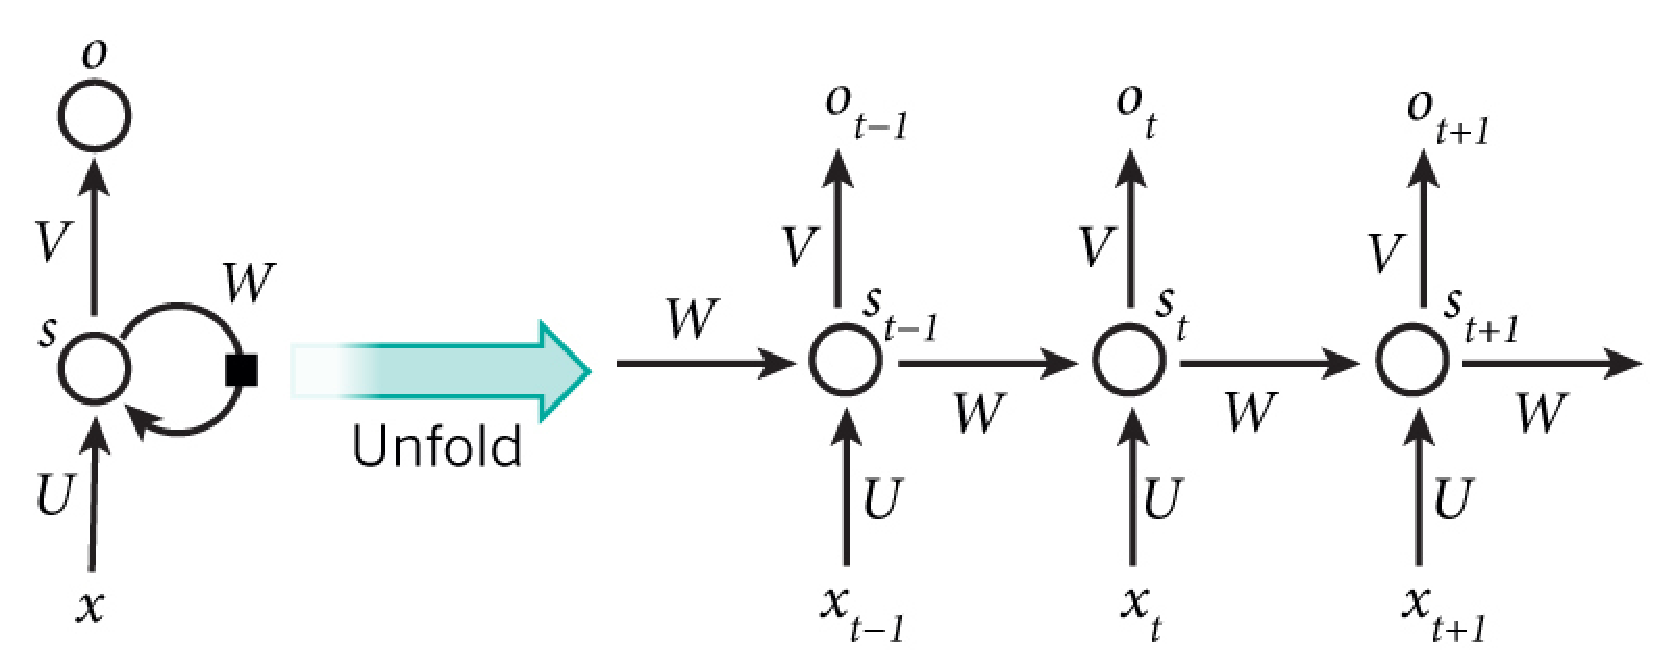
\includegraphics[width=1\textwidth]{bibliography/figure/RNN/RNN.pdf}
        \caption{Một mạng lưới thần kinh tái diễn và sự diễn ra theo thời gian của quá trình tính toán liên quan đến tính toán chuyển tiếp.}
        \label{fig:RNN}
    \end{minipage}

\end{figure}

Mô hình trên mô tả phép triển khai nội dung của một RNN. Triển khai ở đây có thể hiểu đơn giản là ta vẽ ra một mạng nơ-ron chuỗi tuần tự. Ví dụ ta có một câu gồm 5 chữ, thì mạng nơ-ron được triển khai sẽ gồm 5 tầng nơ-ron tương ứng với mỗi chữ một tầng. Lúc đó việc tính toán bên trong RNN được thực hiện như sau:
\begin{itemize}
    \item x\textsubscript{t} là đầu vào tại bước t. Ví dụ, x\textsubscript{t} là một vec-tơ one-hot tương ứng với từ thứ 2 của câu.
    \item s\textsubscript{t} à trạng thái ẩn tại bước t. Nó chính là bộ nhớ của mạng. s\textsubscript{t} được tính toán dựa trên cả các trạng thái ẩn phía trước và đầu vào tại bước đó: s\textsubscript{t} = f(Ux\textsubscript{t} +  Ws\textsubscript{t-1}). Hàm f thường là một hàm phi tuyến tính như tang hyperbolic (tanh) hay ReLu. Để làm phép toán cho phần tử ẩn đầu tiên ta cần khởi tạo thêm \(\theta \).
    \item o\textsubscript{t} à đầu ra tại bước t. Ví dụ, ta muốn dự đoán từ tiếp theo có thể xuất hiện trong câu thì o\textsubscript{t} chính là một vec-tơ xác xuất các từ trong danh sách từ vựng của ta: o\textsubscript{t} = softmax(Vs\textsubscript{t})
\end{itemize}

\subsection{Neural Basis Expansion Analysis for Time Series Forecasting (N-BEATS)}
\vspace{1mm}
\subsection{Tổng quan}
Mô hình N-BEATS, viết tắt của "Neural Basis Expansion Analysis for Time Series Forecasting," được phát triển bởi nhóm nghiên cứu từ Element AI và được công bố trong bài báo năm 2019 bởi Boris Oreshkin và cộng sự.

\subsection{Backcast và Forecast}
Trong N-BEATS, mỗi khối (block) tạo ra hai đầu ra: backcast và forecast. Backcast tái tạo lại dữ liệu đầu vào để mô hình có thể học từ phần dư sau khi trừ đi phần tái tạo này, giúp khối tiếp theo xử lý thông tin còn lại. Forecast là đầu ra dự báo các giá trị tương lai, góp phần vào kết quả cuối cùng.

\subsection{Dữ liệu đầu vào}
N-BEATS làm việc với chuỗi thời gian đơn biến. Đầu vào là một chuỗi thời gian có độ dài $t$:
\[
    x = [y_{T-t+1}, y_{T-t+2}, \ldots, y_T]
\]
Mục tiêu là dự báo giá trị cho $H$ bước tiếp theo:
\[
    y = [y_{T+1}, y_{T+2}, \ldots, y_{T+H}]
\]
Khoảng thời gian xem lại (lookback period) thường có độ dài $t = nH$ với $n$ từ 2 đến 7.

\subsection{Kiến trúc tổng quát}
Mô hình N-BEATS gồm nhiều block xếp chồng lên nhau. Đầu vào của block đầu tiên là dữ liệu $x$. Mỗi block tạo ra hai đầu ra: backcast làm đầu vào cho block kế tiếp, và forecast dùng để tổng hợp dự đoán cuối cùng. Đầu vào của block thứ $i$ (với $i > 1$) là:
\[
    x_i = x_{i-1} - \hat{x}_{i-1}
\]
Dự đoán cuối cùng là tổng hợp các đầu ra forecast của tất cả các block:
\[
    \hat{y} = \sum_{i=1}^{R} \hat{y}_i
\]

\subsection{Kiến trúc của block}
Mỗi block gồm các lớp kết nối đầy đủ (fully connected, FC) với hàm kích hoạt ReLU:
\[
    FC(x_i) = ReLU(Wx_i + b)
\]
Trong đó, $W$ và $b$ là các tham số được học. Mỗi block có $M$ lớp FC chung, sau đó có hai lớp FC để chia đầu ra thành hai nhánh với các hệ số $\theta_f$ và $\theta_b$. Các hệ số này được ánh xạ thành đầu ra backcast và forecast qua các hàm $g_f$ và $g_b$.

\subsection{Các loại block}
\begin{itemize}
    \item \textbf{Generic Block}: Sử dụng các ánh xạ tuyến tính.
    \item \textbf{Trend Block}: Phân tích xu hướng dữ liệu bằng các hàm đa thức bậc thấp:
          \[
              \hat{y}_i = \sum_{j=0}^{p} \theta_{f,j} t^j
          \]
    \item \textbf{Seasonality Block}: Nhận diện tính mùa vụ qua các hàm tuần hoàn, sử dụng chuỗi Fourier:
          \[
              \hat{y}_i = \sum_{j=0}^{H/2 - 1} \theta_{f,j} \cos(2\pi j t) + \theta_{f,j + H/2} \sin(2\pi j t)
          \]
\end{itemize}

\subsection{Long Short Term Memory (LSTM)}
Mạng bộ nhớ dài-ngắn (Long Short Term Memory), thường được gọi là LSTM - là một dạng cải tiến của RNN, nó có khả năng học được các phụ thuộc xa .LSTM gồm trạng thái ẩn \(h_t\) (hidden state) và \(c_t\) (cell state). LSTM gồm 3 thành phần chính:
\begin{figure}[H]
    \centering
    \begin{minipage}{0.25\textwidth}
        \centering
        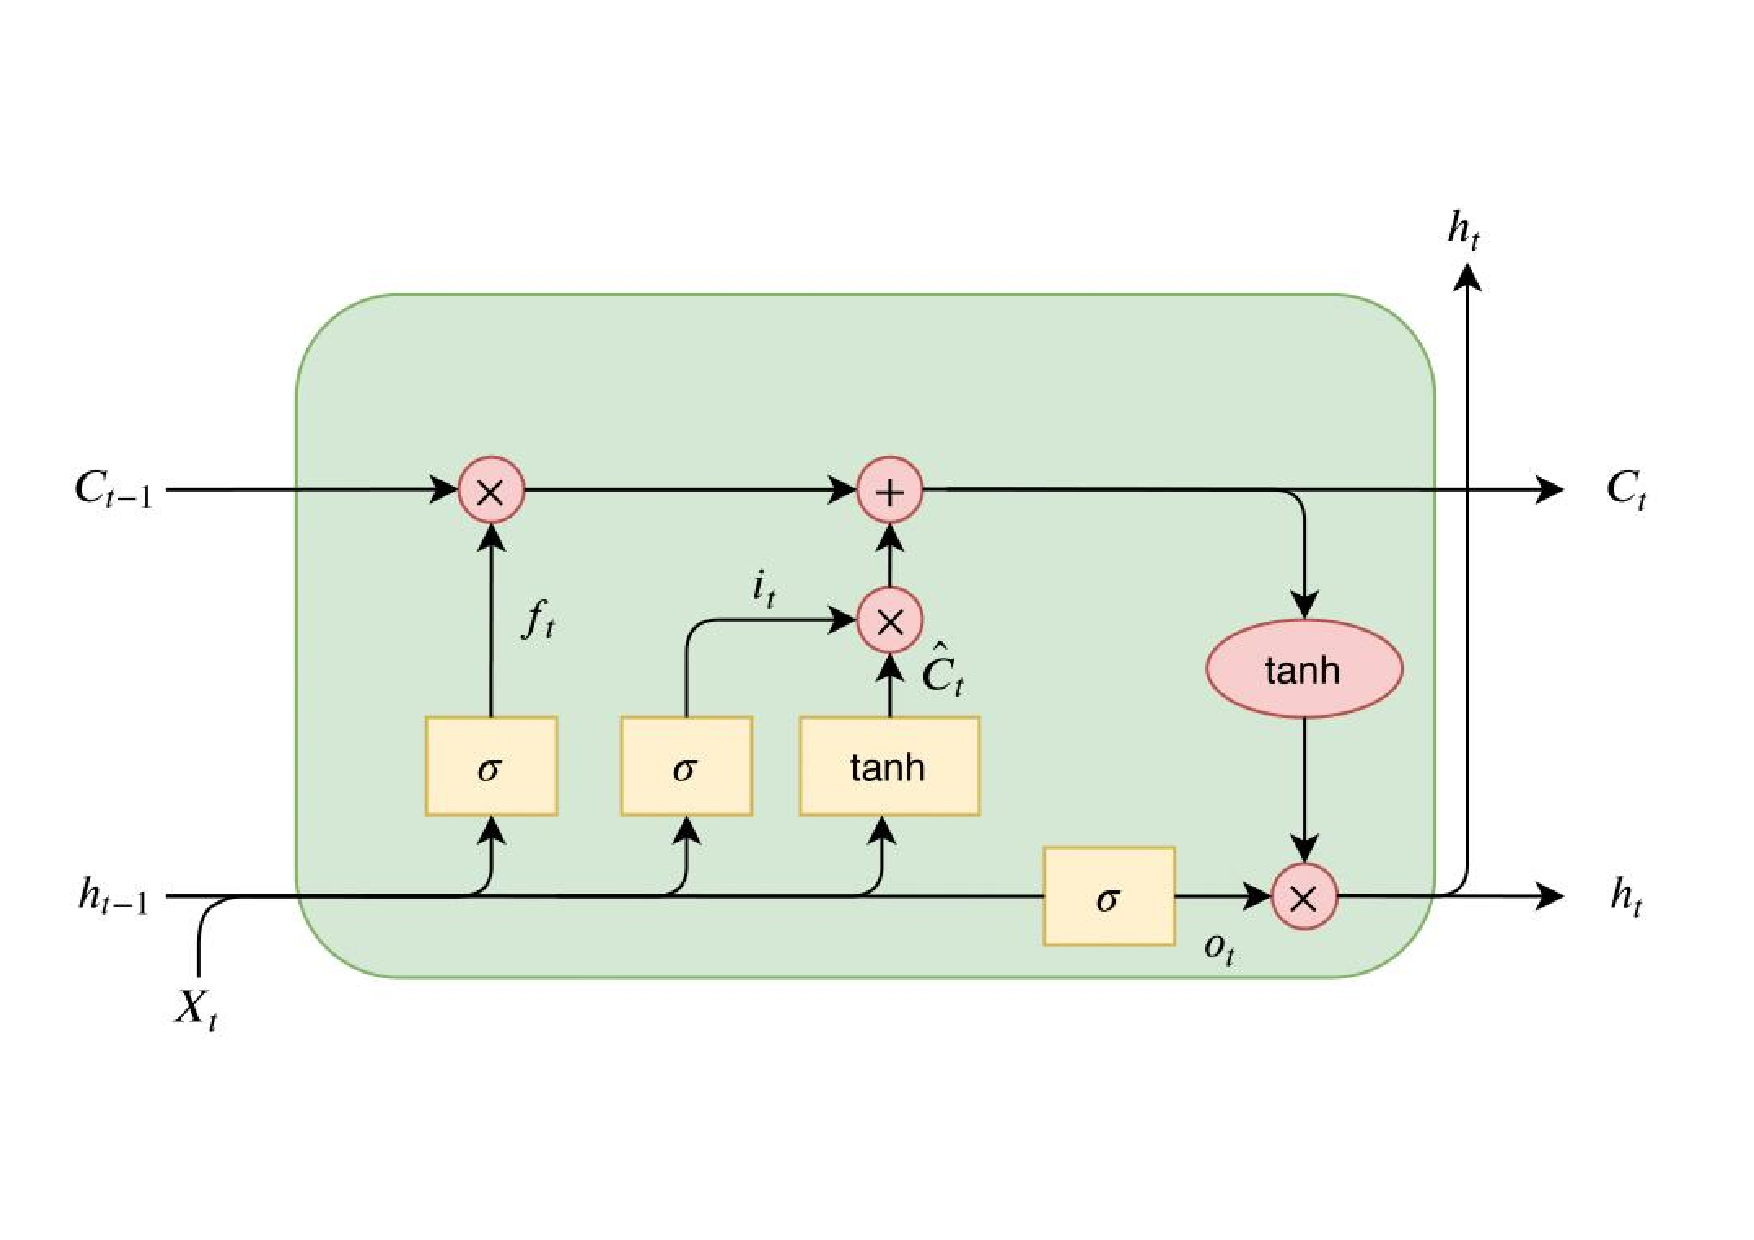
\includegraphics[width=1\textwidth]{bibliography/figure/LSTM/lstm.pdf}
        \caption{Một ô LSTM ở trạng thái t.}
        \label{fig:LSTM}
    \end{minipage}

\end{figure}
Cổng quên(Forget gate):Quản lý việc thông tin đến từ trạng thái trước sẽ được giữ lại hoặc loại bỏ.
\[f_t=\sigma(W_{fx}.x_t+W_{fh}.h_{t-1}+b_f)\]

Cổng vào (Input gate): Quản lý việc học thông tin mới từ đầu vào.
\[i_t=\sigma(W_{ix}.x_t+W_{ih}.h_{t-1}+b_i)\]
\[{\widetilde{C}}_t=tanh\left(W_{cx}.x_t+W_{ch}.h_{t-1}+b_c\right)\]
\[C_t=f_t\circ c_{t-1}+i_t\circ{\widetilde{C}}_t\]

Cổng ra (Output gate): Quản lý việc đưa thông tin mới cập nhật vào trạng thái kế tiếp.
\[o_t=\sigma(W_{ox}.x_t+W_{oh}.h_{t-1}+b_o)\]
\[h_t=o_t\circ tanh(C_t)\]

Trong đó:\\
\indent\textbullet\ \(x_t\) : Vector đầu vào các đặc trưng tại thời điểm t.\\
\indent\textbullet\ \(h_{t-1}\) : Trạng thái ẩn đầu ra của tại thời điểm t-1.\\
\indent\textbullet\ \(W_{fx},W_{fh},W_{ix},W_{ih},W_{cx},W_{hx},\) : Các ma trận trọng số.\\
\indent\textbullet\ \(b_f,b_i, b_c \) : Các hệ số bias.\\
\indent\textbullet\ Tanh: Hàm tanh có giá trị tử -1 đến 1.\\
\indent\textbullet\ \(i_t\) : Giá trị cổng đầu vào tại thời điểm t.\\
\indent\textbullet\ \(\sigma\) : Hàm Sigmoid có giá trị tử 0 đến 1.\\
\indent\textbullet\ \(f_t\) : Giá trị của cổng quên tại thời điểm t.\\
\indent\textbullet\ \(\widetilde{C}_t \) : Ô nhớ mới.\\
\indent\textbullet\ \(C_t \) : Ô nhớ tổng thể.\\
\indent\textbullet\ \(\circ\) : Phép nhân Hadamard.\\
\indent\textbullet\ \(f_t\circ c_{t-1}\) : Quyết định lượng thông tin nào từ trạng thái ô nhớ trước đó sẽ được giữ lại cho ô tiếp theo.\\
\indent\textbullet\ \(i_t\circ{\widetilde{C}}_t\) : Quyết định lượng thông tin nào từ \({\widetilde{C}}_t\) sẽ được thêm vào \(C_t\).\\
\indent\textbullet\ \(o_t \) : Giá trị đầu ra tại thời điểm t.

\subsection{Simple Exponential Smoothing (SES)}
Simple exponential smoothing (SES) hay san bằng hàm mũ đơn giản là một phương pháp dự đoán dữ liệu chuỗi thời gian. SES dựa vào tổng trung bình trọng số của dữ liệu thực tế gần nhất và dữ liệu được dự đoán trước đó để dự đoán dữ liệu tiếp theo trong tương lai. SES phù hợp với dữ liệu chuỗi thời gian không có xu hướng và không có tính mùa vụ.. SES có thể viết ở hai dạng: dạng trung bình trọng số và dạng đối tượng.

Dạng trung bình trọng số:
\[\hat{y}_{t+1|t} = \alpha y_t + (1-\alpha)\hat{y}_{t|t-1}\]

Trong đó:\\
\indent\textbullet\ \(\hat{y}_{t+1|t} \): giá trị dự đoán ở thời điểm t+1 dựa vào giá trị thực tế ở thời điểm t.\\
\indent\textbullet\ \(\alpha\): hệ số làm trơn \((0\le\alpha\le1)\).\\
\indent\textbullet\ \(\hat{y}_{t|t-1} \): giá trị dự đoán ở thời điểm t dựa vào giá trị thực tế ở thời điểm  t-1.\\

Dạng đối tượng:\\
\indent\textbullet\ Phương trình dự đoán: \(\hat{y}_{t+h|t}=l_t\), h=1,2,3,\dots.\\
\indent\textbullet\ Phương trình làm trơn: \(l_t=\alpha y_t+(1-\alpha)l_{t-1}\)\\

Trong đó:\\
\indent\textbullet\ \(\hat{y}_{t+h|t} \): giá trị dự đoán tại thời điểm t+h dựa trên giá trị thực tế ở thời điểm t.\\
\indent\textbullet\ \(\alpha\): hệ số làm trơn \((0\le\alpha\le1)\).\\
\indent\textbullet\ \(\l_t \): cấp độ (giá trị đã được làm trơn) của chuỗi tại thời điểm t.\\
\subsection{Linear Regression}
Phân tích hồi quy là một công cụ để xây dựng các mô hình toán học và thống kê mô tả mối quan hệ giữa một biến phụ thuộc và một hoặc nhiều biến độc lập, hoặc biến giải thích, tất cả đều là các biến số. Kỹ thuật thống kê này được sử dụng để tìm một phương trình dự đoán tốt nhất cho biến \( y \) như một hàm tuyến tính của các biến \( x \).

Một mô hình hồi quy tuyến tính đa biến có dạng:

\[ Y = \beta_0 + \beta_1X_1 + \beta_2X_2 + \cdots + \beta_kX_k + \varepsilon \]

Trong đó:
\begin{itemize}
    \item \( Y \) là biến phụ thuộc (biến mục tiêu).
    \item \( X_1, X_2, \ldots, X_k \) là các biến độc lập (biến giải thích).
    \item \( \beta_0 \) là hệ số chặn.
    \item \( \beta_1, \ldots, \beta_k \) là các hệ số hồi quy cho các biến độc lập.
    \item \( \varepsilon \) là thuật ngữ lỗi.
\end{itemize}

\section{Kết quả}
\subsection{Phương pháp đánh giá}
\textbf{Mean Percentage Absolute Error (MAPE)}: là một phép đo đánh giá mức độ sai lệch tương đối giữa các giá trị dự đoán và giá trị thực tế trong dự đoán
\[
    MAPE = \frac{1}{n} \sum_{i=1}^{n} \left| \frac{y_i - \hat{y}_i}{y_i} \right| \times 100\%
\]

\textbf{Mean Absolute Error (MAE)}: được tính bằng trung bình của sai số tuyệt đối giữa giá trị thực tế và giá trị dự đoán trong tập dữ liệu.
\[
    MAE = \frac{1}{n}\sum_{i=1}^{n}\left|y_i-{\hat{y}}_i\right|
\]
\textbf{Root Mean Square Error (RMSE)}: cho biết mức độ chênh lệch trung bình giữa giá trị dự đoán của mô hình và giá trị thực tế.
\[
    RMSE = \sqrt{\frac{\sum_{i=0}^{N - 1} (y_i - \hat{y}_i)^2}{N}}
\]
\subsection{HaNoi dataset}
\begin{table}[H]
    \centering
    \begin{tabular}{|c|c|c|c|c|}
        \hline
        \multicolumn{5}{|c|}{\textbf{Dataset's Evaluation}}                             \\
        \hline
        \centering Model        & Training:Testing & RMSE    & MAPE (\%)      & MAE     \\
        \hline
        \multirow{2}{*}{ARIMA}  & 7:3              & 49.32   & \textbf{43.87} & 36.28   \\ & 8:2 & 54.44 & 77.00 & 48.37 \\ & \textbf{9:1} & \textbf{31.09} & 49.10 & \textbf{26.47} \\
        \hline
        \multirow{2}{*}{DLM}    & 7:3              & 61.12   & 114.34         & 52.26   \\ & 8:2 & 42.51 & 38.64 & 32.04 \\ & \textbf{9:1} & \textbf{76.20} & \textbf{69.34} & \textbf{61.13}\\
        \hline
        \multirow{2}{*}{GNN}    & 7:3              & 99.755  & 106.15         & 83.293  \\ &  8:2 & 50.950 & 40.74 & 38.152  \\ & \textbf{9:1} &. \textbf{51.968} & \textbf{76.15} & \textbf{46.458}\\
        \hline
        \multirow{2}{*}{GRU}    & 7:3              & 81.263  & 746.699        & 76.353  \\ & 8:2 & 88.876 & 627.15 & 86.025 \\ & \textbf{9:1} & \textbf{84.89} & \textbf{642.77} & \textbf{82.38}\\
        \hline
        \multirow{2}{*}{NBEATS} & 7:3              & 28.31   & 31.20          & 21.95   \\ &8:2 & \textbf{27.26} & \textbf{27.06} & \textbf{21.62} \\ &  \textbf{9:1} & 34.99 & 29.10 & 27.17\\
        \hline
        \multirow{2}{*}{ResCNN} & 7:3              & 28.739  & 31.41          & 20.543  \\ & 8:2 & 32.038	& 30.35 & 24.295\\ & \textbf{9:1} & \textbf{28.718} & \textbf{26.159} & \textbf{21.505}\\
        \hline
        \multirow{2}{*}{RNN}    & 7:3              & 24.9188 & 29.3465        & 10.0873 \\ & 8:2 & 25.7266 & 24.468 & 19.4329 \\ & \textbf{9:1} &  \textbf{27.6262} &	\textbf{29.4822} & 	\textbf{22.0334} \\
        \hline
        \multirow{2}{*}{SES}    & 7:3              & 57.6650 & 49.7333        & 44.0185 \\ & 8:2 & 68.8439 &  61.0638 &  57.1620 \\ & \textbf{9:1} & \textbf{32.0192} & \textbf{26.8332} & \textbf{22.7681}\\
        \hline
        \multirow{2}{*}{LN}     & 7:3              & 64.77   & 59.609         & 51.019  \\ & 8:2 & 65.904 &  58.715 & 54.566 \\ & \textbf{9:1} & \textbf{40.554} & \textbf{33.039} & \textbf{30.327}\\
        \hline
        \multirow{2}{*}{LSTM}   & 7:3              & 26.4712 & 29.8561        & 19.4630 \\ & 8:2 & 27.6927 &  27.0804 &  21.2096 \\ & \textbf{9:1} & \textbf{25.2623} & \textbf{26.7261} & \textbf{19.2388}\\
        \hline
    \end{tabular}
    \vspace{5px}
    \caption{HaNoi Dataset's Evaluation}
    \label{mbbresult}
\end{table}
\begin{thebibliography}{00}
    \bibitem{b1} Ke, Z., Zhang, J., \& Wen, Z. (2023). Gauss-Newton Temporal Difference Learning with Nonlinear Function Approximation.
    \bibitem{b2} H. Choi, C. Jung, T. Kang, H. J. Kim, and I. -Y. Kwak, "Explainable time-series prediction using a residual network and gradient-based methods," in IEEE Access, vol. 10, pp. 108469-108482, 2022.
    \bibitem{b3} Doan Vo Duy Thanh, Nguyen Van Cuong, Vo Tan Phat, Le Khac Hong Phuc, Nguyen Duy Du, Nguyen Van Quang, Pham Minh Duc, Pham Hong Vinh, and Nguyen Canh Thuong. \textit{Gated Recurrent Unit (GRU)}. Accessed May 26, 2024. \url{https://d2l.aivivn.com/chapter_recurrent-modern/gru_vn.html}.
    \bibitem{b4} Nejedly P, Ivora A, Viscor I, Koscova Z, Smisek R, Jurak P, Plesinger F. Classification of ECG using ensemble of residual CNNs with or without attention mechanism. Physiol Meas. 2022 Apr 28;43(4). doi: 10.1088/1361-6579/ac647c. PMID: 35381586.
    \bibitem{b5} M. Chiogna and C. Gaetan, "Dynamic Generalized Linear Models with Application to Environmental Epidemiology," Journal of the Royal Statistical Society Series C: Applied Statistics, vol. 51, no. 4, pp. 453-468, 2002.
    \bibitem{b6} D. Osthus, P. C. Caragea, D. Higdon, S. K. Morley, G.D.Reeves and B. P. Weaver, "Dynamic linear models for forecasting of radiation beltelectrons and limitations on physical interpretationof predictive models," vol. 12, no. 6, pp. 323-446, 2014.
    \bibitem{b7} Wang, Junjie \& Su, Xiaohong \& Zhao, Lingling \& Zhang, Jun. (2020). Deep Reinforcement Learning for Data Association in Cell Tracking. Frontiers in Bioengineering and Biotechnology. 8. 298. 10.3389/fbioe.2020.00298.
    \bibitem{b8} Rajnish Rakholia , Quan Le, Bang Quoc Ho, Khue Vu, Ricardo Simon Carbajo. “Multi-output machine learning model for regional air pollution forecasting in Ho Chi Minh City, Vietnam” (2023). doi: \url{https://doi.org/10.1016/j.envint.2023.107848}. URL: \url{https://www.sciencedirect.com/science/article/pii/S0160412023001216}
    \bibitem{b9} Nguyen Anh Tuan, Le Anh Ngoc . “APPLYING N-BEATS MODEL FOR SHORT-TERM LOAD FORECASTING IN VIETNAM” (2022). URL: \url{https://khcncongthuong.vn/tin-tuc/t18804/ung-dung-mo-hinh-n-beats-cho-du-bao-phu-tai-dien-ngan-han-o-viet-nam.html}
    \bibitem{b10} B. S, Freemana, G. Taylora, B. Gharabaghia and J. Thé, "Forecasting air quality time series using deep learning," Journal of the air \& waste management association, vol. 68, no. 8, pp. 866-886, 2017-2018.
    \bibitem{b11} Fatima, Samreen \& Saad, Sayed \& Zia, Syeda \& Hussain, Ehtesham \& Fraz, Tayyab \& Shafi, Mehwish \& Khan,. (2019). Forecasting Carbon Dioxide Emission of Asian Countries Using ARIMA and Simple Exponential Smoothing Models. International Journal of Economic and Environment Geology. 10. 10.46660/ojs.v10i1.219.
    \bibitem{b12} Navares, Ricardo \& Aznarte, José. (2019). Predicting air quality with deep learning LSTM: Towards comprehensive models. Ecological Informatics. 55. 101019. 10.1016/j.ecoinf.2019.101019.
    \bibitem{b13} Jarrett, Jeffrey E., and Eric Kyper. "ARIMA modeling with intervention to forecast and analyze chinese stock prices." International Journal of Engineering Business Management 3.3 (2011): 53-58.
    \bibitem{b14} Devi, B. Uma, D. Sundar, and P. Alli. "An Effective Time Series Analysis for Stock Trend Prediction Using ARIMA Model for Nifty Midcap-50."
    \bibitem{b15} Tseng, Fang-Mei, et al. "Fuzzy ARIMA model for forecasting the foreign exchange market." Fuzzy sets and systems 118.1 (2001): 9-19
    \bibitem{b16} Contreras, J., Espinola, R., Nogales, F. J., \& Conejo, A. J. (2003). ARIMA models to predict next-day electricity prices. Power Systems, IEEE Transactions on, 18(3), 1014-1020.
    \bibitem{b17} Oreshkin, B. N., Carpov, D., Chapados, N., \& Bengio, Y. (2019). N-BEATS: Neural basis expansion analysis for interpretable time series forecasting. arXiv preprint arXiv: 1905.10437. \url{https://doi.org/10.48550/arXiv.1905.10437}.
    \bibitem{b18} Loganathan, A. \& Palraj, Sumithra \& V, Deneshkumar. (2022). Estimation of Air Quality Index Using Multiple Linear Regression. Applied Ecology and Environmental Sciences. 10. 717-722. 10.12691/aees-10-12-3.
\end{thebibliography}

\end{document}
